% Chapter Template
%!TEX root=../main.tex

\chapter{Theory} % Main chapter title

\label{Chapter2} % Change X to a consecutive number; for referencing this chapter elsewhere, use \ref{ChapterX}

\lhead{Chapter 2. \emph{Theory}} % Change X to a consecutive number; this is for the header on each page - perhaps a shortened title
\begin{doublespace}

The equations presented in this chapter as well as the derivation of drift diffusion equations form a basis for simulating coupled ionic-electronic devices. First, \tjs{the} Boltzmann transport equation which is the starting point for generating the drift diffusion equation is introduced. The introduction of \tjs{the} Boltzmann transport equation is followed by the derivation of \tjs{the} drift diffusion equation and the presentation of the set of equations that describe the behavior of a coupled ionic-electronic device. The last part of the chapter shows analytic solutions to \tjs{the} drift diffusion equations which are used to test the numerical methods derived in chapter 4.   

\section{Carrier Transport Equations}
Drift diffusion equations, which are based on Boltzmann Transport Equations (BTE) \cite{Dragica1}, need to be solved in order to model the complex behavior of an ionic electronic device. The drift diffusion equations used are derived by simplifying \tjs{the} BTE equation via approximations. These simplifications dictate the limits of the drift-diffusion model, therefore they need to be well understood.

The derivation of \tjs{the} Boltzmann transport equation starts by stating that a distribution of charged particles can be defined by their position in space \textbf{r} and momentum \textbf{k} in time \textbf{t} using a probability distribution function $f(k,r,t)$. This results in the most general form of \tjs{the} Boltzmann transport equation\cite{snowden}.

\begin{equation}
\frac{d }{dt}f(k,r,t)=0
\end{equation}

This general form of BTE needs to be expanded and relevant physical equations need to be incorporated to get an equation describing a specific problem or a device. 
Many different device simulators use some sort of approximation to \tjs{the} BTE. In commercial semiconductor simulators drift diffusion equations are commonly used to describe the movement of charge carriers such as holes ($p$) and electrons ($n$) in a material\cite{Comsol}\cite{SILVACO}\cite{LumDev}. 

After this brief introduction to \tjs{the} BTE, rather than going through the mathematical derivation of the drift diffusion model, the approximations that are made along the process of derivation are discussed in order to get a better insight on the model. The approximations and equations presented in this chapter is based on C.M Snowden's book called ``Semiconductor Device Modeling''\cite{snowden}. It must be noted that the following derivation is only true for isotropic media but it can be extended to accommodate anisotropic media by using appropriate tensor equations for carrier mobilities and diffusivities.

As a particle travels in a solid state device it collides with other particles as well as the atoms in the device. For \tjs{the} drift-diffusion equations individual lattice scattering events or collisions are averaged and all the particles have an average constant \tjs{drift} velocity under the effects of an electric field \cite{snowden}. The movement of the particles due to the electric field is called the drift current. The relationship between the drift velocity and the electric field is given by the following equation:
\begin{equation}
v=\mu E
\end{equation}
$\mu$ is called the mobility and it determines the \tjs{average} speed at which the particles \tjsr{are going to}{} move when subject to an electric field. Mobility of a particle can be a function of \tjsr{different}{} variables such as temperature or the electric field. Drift current density can be derived based on \tjs{the} drift velocity\cite{snowden}.
\begin{equation}
J_E=q n\mu E=q n v 
\end{equation}
Where q is the elementary charge and n is the electron density. In addition to the previous assumptions, it is assumed that the lattice is perfectly uniform, has a uniform temperature distribution and all the temperature of the particles are close to the temperature of the lattice. Therefore, all the particles are assumed to have the same thermal velocity ($v_{th}$) and mean free path ($l_f$). These quantities can be combined into one single coefficient called the diffusion constant,
\begin{equation}
D=v_{th} \;l_f
\end{equation}
\tjs{The} Drift and diffusion coefficients are related to each other via the Einstein relationship\cite{snowden}:
\begin{equation}
D=\frac{\mu k T}{q}
\end{equation}
Where $k$ is the Boltzmann constant and $T$ is the lattice temperature. The random thermally driven motion produces diffusion and results in a second term which contributes to the carrier movement and it is called the diffusion current density,
\begin{equation}
J_D=qD\frac{dn}{dx}
\end{equation}
Unlike the drift current density, which is directly related to the carrier density, diffusion current density is related to the carrier density's first order derivative in space. Combining these two terms results in the following the current density equation for electrons in one dimension,
\begin{equation}
\vec{J_n^x}=q \mu_{n} n \vec{E_x}+qD_{n} \frac{dn}{dx} 
\label{cdenn}
\end{equation}
This equation can be easily extended to other dimensions by simply using the appropriate terms:
\begin{equation}
\vec{J_n^y}=q \mu_{n} n \vec{E_y}+qD_{n} \frac{dn}{dy} 
\end{equation}

The current density equations can be used for both positively and negatively charged particles by changing the sign of the diffusion current density.
\begin{equation}
\vec{J_p^x}=q \mu_{p} p \vec{E_x}-qD_{p} \frac{dp}{dx} 
\label{cdenp}
\end{equation}
Anisotropic drift and diffusion coefficients can be handled with ease by using different coefficients for different directions. Also the mobility and the diffusivity can be a function of any variable such as position or temperature.

Current density equations by themselves are not enough to solve this time dependent problem. It is necessary to account for the movement of charge over time which is captured in the continuity equation. It is a statement of conservation of particle density over time. The change in the amount of carriers over time in a particular area must be equal to the difference in current density over the same area. Additionally the amount of charge can change due to generation-recombination of charged particles. The continuity is captured by equations:
\begin{equation}
\frac{\partial n}{\partial t}=\frac{1}{q}\nabla \cdot \vec{J_n}+U_{n}
\label{conn}
\end{equation}
\begin{equation}
\frac{\partial p}{\partial t}=-\frac{1}{q}\nabla \cdot \vec{J_p}+U_{p}
\label{conp}
\end{equation}
$U_{n}$ and $U_{p}$ are net generation recombination rates.  

Electric field can be generated in two different ways. One is through the distribution of net charge over the area and the other one is an externally applied potential. It is possible to calculate the potential distribution over an area by using Poisson's equation \cite{Dragica1},
\begin{equation}
\nabla \cdot  (\varepsilon \nabla V)=-\rho
\label{poisson}
\end{equation}
Where the variables \textit{$\varepsilon$}, \textit{V}, \textit{$\rho$} are permittivity, electric potential and charge density respectively. Once the electric potential is known the electric field can be obtained by just calculating the negative gradient of the electric potential,
\begin{equation}
\vec{E}=-\nabla V
\label{Efield}
\end{equation}

The electric field can be split into multiple components depending on the dimensions of the problem. In a 2-D case they are $\vec{E_x}$ and $\vec{E_y}$.
\begin{equation}
\vec{E_x}=-\hat{x}\frac{\partial V}{\partial x}
\end{equation}
\begin{equation}
\vec{E_y}=-\hat{y}\frac{\partial V}{\partial y}
\end{equation}
Once the electric field and the current density are known, the current can be easily calculated by using the following integral \cite{snowden},
\begin{equation}
I=\int\limits_{s}^{}\vec{J_{tot}} \cdot ds = \int\limits_{s}^{}(J_n+J_p+\varepsilon\frac{\partial E}{\partial t})ds
\end{equation}

Poisson's equation and drift-diffusion equations are coupled through the electric field and net charge distribution. The strength of this non-linear coupling depends on the size of the device and the charge density which determines the total amount of charge over an area. In a strongly coupled system of differential equations, small changes in either the charge density or the electric field can easily cause instabilities in the simulation. This is further discussed in the next chapter while developing a numerical scheme to solve the system of equations described in this chapter. 

The main equations for the drift-diffusion model that are used for the coupled electronic-ionic simulation can be compactly written as:
\begin{equation}
\nabla \cdot  (\varepsilon \nabla V)=-q(p-n+N_{c}-N_{a}+N_{f})
\end{equation}
\begin{equation}
\vec{J_p}=q\mu_p p \vec{E}-q D_p \nabla p
\end{equation}
\begin{equation}
\vec{J_n}=q\mu_n n \vec{E}+q D_n \nabla n
\end{equation}
\begin{equation}
\vec{J_{N_{a}}}=q\mu_{N_{a}} N_{a} \vec{E}+q D_{N_{a}} \nabla N_{a} 
\end{equation}
\begin{equation}
\vec{J_{N_{c}}}=q\mu_{N_{c}} N_{c} \vec{E}-q D_{N_{c}} \nabla N_{c}
\end{equation}
\begin{equation}
\frac{\partial p}{\partial t}=-\frac{1}{q}\nabla \cdot \vec{J_p}  + U_{p}
\end{equation}
\begin{equation}
\frac{\partial n}{\partial t}=\frac{1}{q}\nabla \cdot \vec{J_n}+ U_{n}
\end{equation}
\begin{equation}
\frac{\partial N_{a}}{\partial t}=\frac{1}{q}\nabla \cdot \vec{J_{N_{a}}} + U_{N_{a}}
\end{equation}
\begin{equation}
\frac{\partial N_{c}}{\partial t}=-\frac{1}{q}\nabla \cdot \vec{J_{ N_{c} }}+ U_{N_{c}}
\end{equation}

This system of equations consist of 4 different mobile charged particles, holes (\textit{p}), electrons (\textit{n}), cations (\textit{$N_{c}$}) and anions (\textit{$N_{a}$}). \textit{$N_{f}$} is used for fixed charge which can be positive or negative depending on the device. \textit{U} is used for the generation recombination term of each mobile charge carrier. The particles are coupled to each other through Poisson's equation since they all carry electric charge. \tjs{A} drift diffusion model does not limit the \tjsr{amount}{number} of mobile particles that can be simulated in a device. So this model can be easily modified to accommodate any number of mobile species based on what is physically present in a device. Even after many approximations to the BTE, the drift diffusion equations have analytical solutions for only few isolated cases. The analytical solutions developed in the rest of this chapter are used in the testing of the numerical method developed for simulating a memristor. 

\section{Analytic Solutions}

Three different analytic solutions to drift diffusion equations are developed in this section. \tjsr{It starts with}{Initially} a simple steady state problem with uniform electric field \tjs{is solved}. The second example, which is more complex than the first one, is a transient solution for a charge distribution moving under uniform electric field. Finally, a PN junction problem is solved which incorporates the drift diffusion equation with Poisson's equation and provides a steady state solution for electron/hole density distributions, electric potential and electric field. 
  
\subsection{Steady State Solution Over a Finite Domain}

The problem that will be solved in this section consists of a finite amount of charge and a uniform electric field pushing this charge against a wall. It is assumed that the charge density is low enough not to affect the uniform electric field, therefore the solution of Poisson's equation is not necessary. To simplify the problem even further only a steady state solution is derived. Also it is important to note that the initial distribution of the charge density does not matter in this problem since all the charge will be redistributed in steady state. The only relevant information is the total amount of charge subject to the electric field. At steady state, drift and diffusion currents are in equilibrium and net current density is zero. The following equation shows the hole current density at equilibrium:
\begin{equation}
J_p(x)=q \mu_{p} p E-qD_{p} \frac{dp}{dx} =0
\end{equation}
Total current density will only be zero when the drift current density generated by the electric field is completely balanced by the diffusion current density \tjs{leading to:}
\begin{equation}
q \mu_{p} p E=qD_{p} \frac{dp}{dx}
\end{equation}
\tjs{which can be rearranged to be,}
\begin{equation}
 \frac{\mu_{p} E}{D_{p}} p  = \frac{dp}{dx}
 \label{pdif}
\end{equation}
This is a simple differential equation that can be solved by assuming that hole density has the following form:
\begin{equation}
p(x)=Ce^{ax}
\label{px}
\end{equation}
\textbf{C} and \textbf{a} are arbitrary constants. Equation \eqref{px} can be placed into \eqref{pdif},
\begin{equation}
 \frac{\mu_{p} E}{D_{p}} Ce^{ax}  = a Ce^{ax}
\end{equation}
\tjs{solving for $a$ we have,}
\begin{equation}
a=\frac{\mu_{p} E}{D_{p}}
\end{equation}

A general form for the solution is generated by placing $a$ back into equation \eqref{px} \tjs{giving,}
\begin{equation}
p(x)=Ce^{\frac{\mu_{p} E}{D_{p}}x}
\label{p_ss}
\end{equation}
It is possible to solve for \textbf{C} by observing that the total amount of charge at steady state must be equal to the initial amount of charges since all the holes remain inside the conductor. So the integral of the initial hole density distribution must be equal to the integral of the charge density at steady state,
\begin{equation}\nonumber
\int\limits_{0}^{L}Ce^{\frac{\mu_{p} E}{D_{p}}x}dx=\int\limits_{0}^{L}p(t=0,x)dx
\end{equation}
\tjs{Which can be solved for $C$,}
\begin{equation}
	% \nonumber
C=\frac{\int\limits_{0}^{L}p(t=0,x)dx}{\int\limits_{0}^{L}e^{\frac{\mu_{p} E}{D_{p}}x}dx}
% \end{equation}
% \begin{equation}
% C
=\frac{\int\limits_{0}^{L}p(t=0,x)dx}{\frac{D_p}{\mu_p E}[e^{\frac{\mu_p E}{D} L} -1]}
\label{p_ss_c}
\end{equation}

Equation \ref{p_ss} combined with equation \ref{p_ss_c} gives a complete solution for this problem. \tjsr{which}This solution shows that increasing the electric field will \tjsr{concentrate}{increase} the \tjs{concentration of} charge density at the edge of the conductor. Physically this behavior is reasonable, since the force that is pushing the particles against a wall is getting greater and it is making the charges accumulate even more. The following plot demonstrates the effect of the electric field on the hole distribution.
\begin{figure}[!htp]
\centering
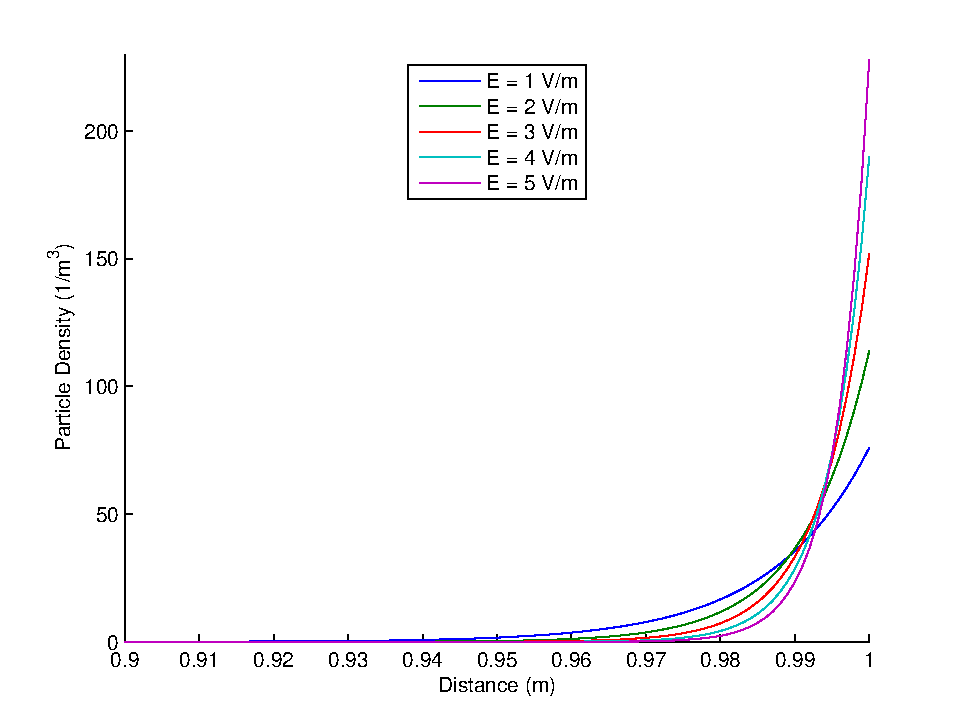
\includegraphics[scale=0.65]{AnalyticSS}
\caption{Increased accumulation of particles due to increased electric field} 
\end{figure}

\tjs{This phenomenon is related to Debye screening which is characterized by the Debye length.} The Debye length is the length over which mobile charge carriers screen out an external electric field and it determines how steeply charges will accumulate over a certain distance and it can be calculated using the following equation\cite{Dragica1}:
\begin{equation}
L_D=\sqrt{\frac{\varepsilon V_{th}}{q n}}
\end{equation}
Where the variables \textit{$V_{th}$}, \textit{n} and \textit{$\varepsilon$} are thermal voltage, particle density and permittivity respectively. This example also illustrates the decrease in the Debye length due to the increase in the charge density. Debye length is determined by the strength of the electric field created by the charge present in the material. The increase in the electric field in this example is analogous to the increase in charge density. Increased charge density creates a larger electric field. This creates a steeper accumulation of the charged particles and a decrease in the Debye length. 


\subsection{Transient Solution Over an Infinite Domain}

The problem that is solved in this section is based on Haynes-Shockley experiment\cite{1949PhRv...75..691H} and consists of an initial particle density distribution subject to a uniform electric field over an infinitely long conductor. The charge distribution drifts and diffuses over time. This requires a transient solution \tjs{and} therefore the continuity equation (\ref{conn}) needs to be solved. Again, it is assumed that charged particles do not affect the electric field since their density is low enough , therefore solution of Poisson's equation is not necessary. 

The first step of the solution process is the insertion of \eqref{cdenn} into \eqref{conn}.
\begin{equation}
\frac{\partial n}{\partial t} = \frac{1}{q}\nabla \cdot (q \mu_{n} n \vec{E}+qD_{n} \frac{dn}{dx} )
\end{equation}

For 1-D this can be simplified to:
\begin{equation}
\frac{\partial n}{\partial t} = \mu_n E \frac{d n}{d x}+D_{n}\frac{d^{2}n}{dx^{2}}
\label{adifg}
\end{equation}
Using separation of variables the solution can be separated into time and space dependent functions\cite{NumModel},
\begin{equation}
n(t,x)=n(t)n(x)=n_t n_x
\label{adifn}
\end{equation}
Placing equation \eqref{adifn} into \eqref{adifg} and dividing by \textit{n(t,x)},
\begin{equation}
\frac{1}{n_{t}}\frac{d n_{t}}{d t}=\mu_n E \frac{1}{n_{x}}\frac{d n_{x}}{dx}+D\frac{1}{n_{x}}\frac{d^2 n_{x}}{dx^2}
\label{Adif}
\end{equation}
Assuming both sides of the equation are equal to a constant \textit{-k}, the time dependent part of the problem becomes a simple first order differential equation.
\begin{equation}
\nonumber
\frac{1}{n_{t}}\frac{d n_{t}}{dt}=-k
\end{equation}

\begin{equation}
\nonumber
\frac{d n_{t}}{d t}=-kn_t
\end{equation}

Based on the above differential equation $n_t$ can take the following form:
\begin{equation}
n_t=C_1 e^{-kt}
\label{nt}
\end{equation}
\tjsr{Now}{With} for $n_x$ assuming a solution of the form below,
\begin{equation}
n_x=C_2 e^{-j\omega x}
\label{nx}
\end{equation}

Placing \eqref{nx} into \eqref{Adif} \tjs{we obtain,}
\begin{equation}
\omega^2 D C_2 e^{-j\omega x}-j\omega \mu_n E C_2 e^{-j\omega x}+kC_2e^{-j\omega x}=0
\label{omegak}
\end{equation}
Simplifying equation \eqref{omegak} and solving for k gives,
\begin{equation}
k=\omega^2 D+j\omega \mu_n E
\label{k}
\end{equation}

Combining equation \eqref{nt}, \eqref{nx} and \eqref{k} to get the initial form of the solution. $(C=C_1C_2)$
\begin{equation}
n=n_tn_x=Ce^{(-\omega^2 D + j\omega \mu_n E)t} e^{-j\omega x}
\end{equation}
The application of the superposition principle\cite{DifEq} leads to:
\begin{equation}
n=n_tn_x=\int\limits_{-\infty}^{\infty}C(\omega)e^{(-\omega^2 D + j\omega \mu_n E)t} e^{-j\omega x}d\omega
\label{nfinal1}
\end{equation}

The distribution of $n_x$ is known at t=0.
\begin{equation}
n(x,t=0)=\int\limits_{-\infty}^{\infty}C(\omega) e^{-j\omega x}d\omega
\end{equation}
$C(\omega)$ is \tjsr{just}{} the inverse Fourier transform of $n(x,0)$,
\begin{equation}
C(\omega)=\int\limits_{-\infty}^{\infty}n(x,0)e^{j\omega x}dx
\label{comega}
\end{equation}

The final form of the solution is generated by placing equation \eqref{comega} into \eqref{nfinal1}:
\begin{equation}
n=\int\limits_{-\infty}^{\infty}\int\limits_{-\infty}^{\infty}n(z,0)e^{j\omega z}dz e^{(\omega ^2 D-j\omega \mu_n E)t}e^{j\omega x}d\omega
\label{nfinal2}
\end{equation}

Rearranging equation \eqref{nfinal2},
\begin{equation}
n=\int\limits_{-\infty}^{\infty}\int\limits_{-\infty}^{\infty}n(z,0) e^{(\omega ^2 D-j\omega \mu_n E)t}e^{j\omega x} e^{j\omega z}  dz d\omega
\end{equation}
Using a Gaussian initial distribution results in\tjsr{to}{}:
\begin{equation}
n(x,0)=e^{- (\frac{x-x_o}{\sigma})^2}
\end{equation}
Which leads to,
\begin{equation}
n(x,t)=\frac{1}{\sqrt{4D_nt+\sigma^{2}}}e^{-\frac{(t\mu_n E-x+x_o)^2}{4D_n t+\sigma^2}}
\end{equation}

If the initial distribution is a rectangular then the solution takes the following form:

\begin{equation}
n(x,t)=\frac{1}{2} erf(\frac{w+2t \mu_n E-2x}{4\sqrt{D_n t}})-\frac{1}{2}erf(\frac{-w+2t \mu_n E-2x}{4\sqrt{D_n t}}) 
\end{equation}

Following plots show the evolution of two particle densities with \tjs{the} different initial distributions described above.

\begin{figure}[!htp]
\centering
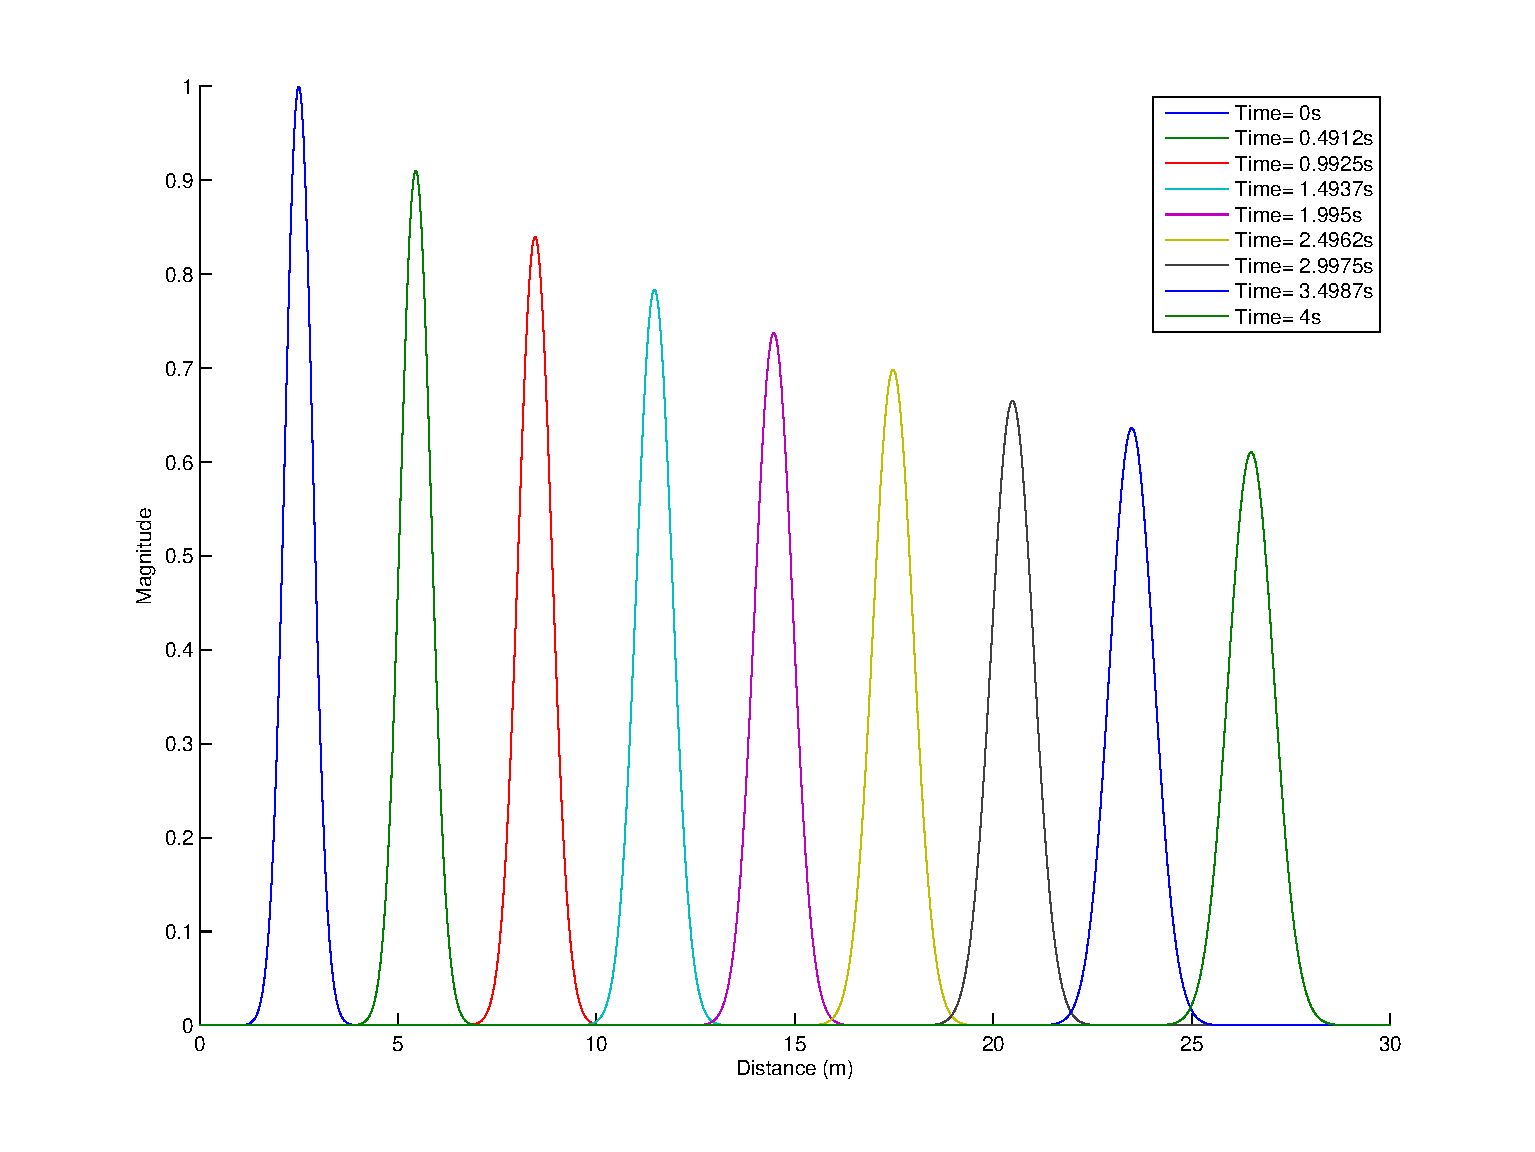
\includegraphics[scale=0.5]{AnalyticGauss}
\caption{A Gaussian particle density distribution drifting and diffusing over time} 
\end{figure}

\begin{figure}[!htp]
\centering
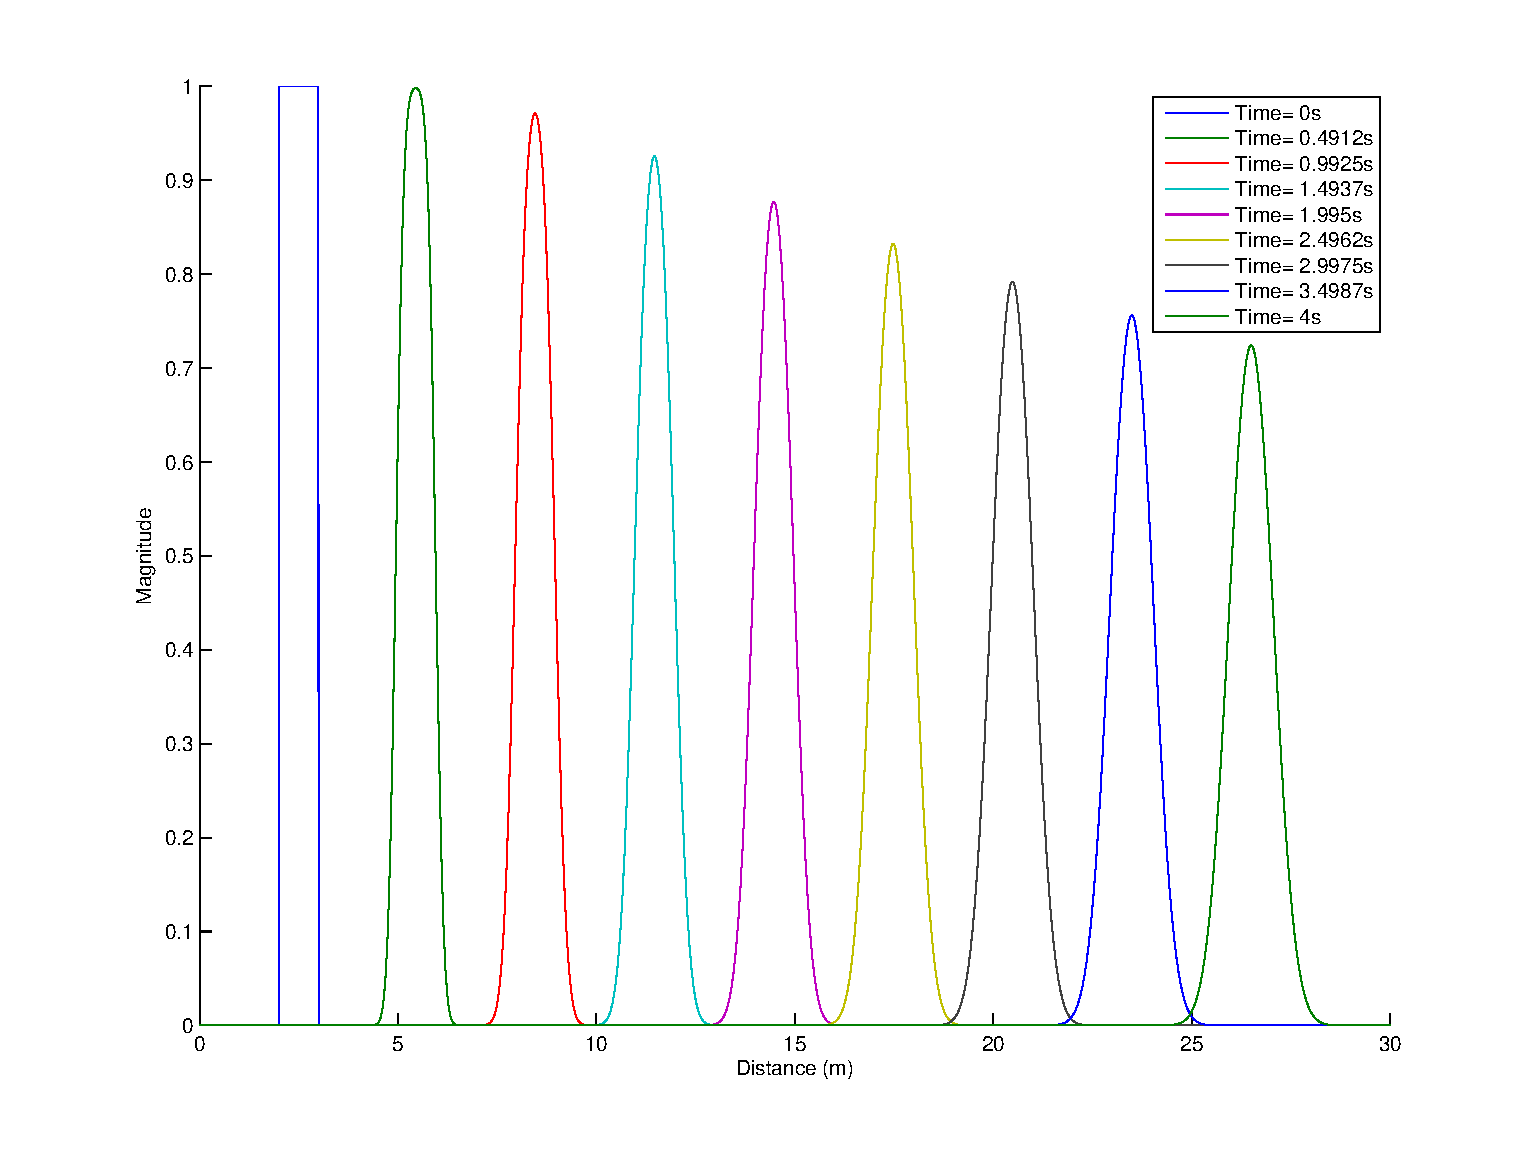
\includegraphics[scale=0.5]{AnalyticRect}
\caption{A rectangular particle density distribution drifting and diffusing over time} 
\end{figure}
\clearpage
\subsection{PN Junction}
The previous analytical solutions involved the solution of Poisson's equation and the continuity equation which \tjsr{are}{were assumed to be} not coupled. An example where these equations are tightly coupled is examined in this section. There are usually no direct analytical solutions for coupled equations but it is possible to get a closed form solution by making use of certain approximations. One example of this situation is an abrupt p-n junction. The derivation for an abrupt junction presented in this section is mostly based on the book ``Physics of Semiconductor Devices'' written by Kwok K. Ng et al. \cite{Physem}. 

An abrupt p-n junction is created when two materials of opposite doping, p-type and n-type, are brought together. For this example the p-type material has a net hole concentration of $N_{A}$ and the n-type materials has a net electron concentration of $N_{D}$. The junction is defined at the interface where $N_A=N_D$ \cite{Physem}. 

\begin{figure}[!htp]
\centering
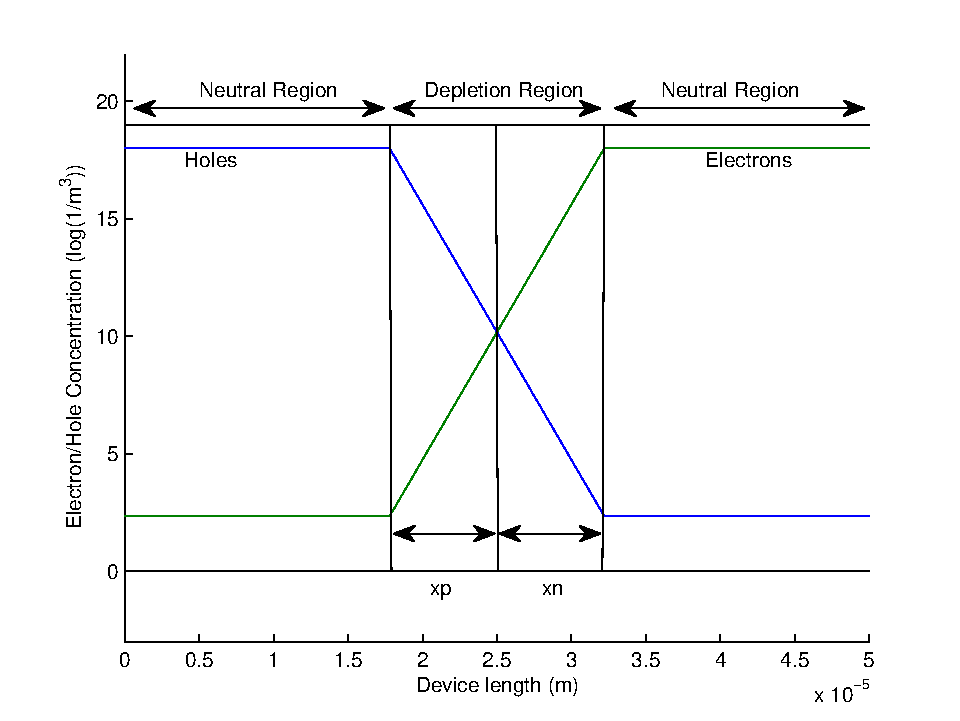
\includegraphics[scale=0.8]{3331}
\caption{PN junction electron/hole density} 
\end{figure}

In this example an analytical solution for an abrupt p-n junction is derived. To \tjsr{get}{obtain} a solution for this problem  \tjs{the} depletion region approximation is used. This approximation starts by assuming that the charges are fully depleted around the junction\cite{Physem}. All the electric field is confined in the depletion region and regions far away from the junction are neutral. Based on this, the net charge density over the entire region is:
\begin{equation}
\frac{d \vec{E} }{dx}=\frac{\rho}{\varepsilon}=\frac{q}{\varepsilon}(-N_{A}+N_{D})
\end{equation}
\tjs{with,}
\begin{equation}
\rho = \begin{cases}
         0 & \text{for} \;  x<-x_{p}\\
       -qN_{A} & \text{for}  -x_{p}\leq x \leq 0 \\
        qN_{D} & \text{for} \; 0 \leq x \leq< x_{n}  \\
        0 & \text{for}\;  x>x_{n} \\
     \end{cases}
\end{equation}

The electric field over the entire region can be calculated by integrating $\rho$,
\begin{equation}
E = \begin{cases}
       \int \frac{-qN_{A}}{\varepsilon}  dx+ C_{1} & \text{for}  -x_{p}\leq x \leq 0 \\
       \int \frac{qN_{D}}{\varepsilon} dx+ C_{2}   & \text{for } \; 0 \leq x \leq x_{n}  \\
     \end{cases}
\end{equation}
It is possible to solve for $C_{1}$ and $C_{2}$ since electric field must go to zero at $x_{p}$ and $x_{n}$,
\begin{eqnarray}
E(x=-x_{p}) & = 0  \; \;  \Rightarrow  \;\; C_{1}= \frac{-qN_{A}}{\varepsilon}x_{p}\nonumber \\
E(x=x_{n}) & =0  \; \;  \Rightarrow  \;\; C_{\tjsr{}{2}}= \frac{qN_{D}}{\varepsilon}x_{n}
\label{pn_efield}
\end{eqnarray}

Then \textit{E(x)} becomes:
\begin{equation}
E(x) = \begin{cases}
         \frac{-qN_{A}}{\varepsilon}(x+x_{p}) & \text{for}  -x_{p}\leq x \leq 0 \\
         \frac{qN_{D}}{\varepsilon}(x-x_{n})  &  \text{for} \; 0 \leq x \leq x_{n}  \\
     \end{cases}
\end{equation}
Additionally, the electric field must be continuous across the interface therefore the electric field in the p-type side and the n-type side must equal each other at the interface or when \textit{x = 0} \tjs{giving,}
\begin{equation}
\frac{-qN_{A}}{\varepsilon}(x_{p})=\frac{qN_{D}}{\varepsilon}(-x_{n}) \nonumber
\end{equation}
\begin{equation}
N_{A}x_{p}=N_{D}x_{n}
\label{NAeqND}
\end{equation}

This equation states that the total charge on one side of the junction must be the same as the total charge on the other. In other words, the net charge on each side keeps the electric field confined to the depletion region.

To find the voltage as a function of distance, equation \ref{pn_efield} can be integrated,
\begin{equation}
V(x) = \begin{cases}
       \int -E(x)dx=\int \frac{qN_{A}}{\varepsilon}(x+x_{p}) dx = \frac{qN_{A}}{\varepsilon}(\frac{x}{2}+x_{p})+ C_{3} & \text{for}  -x_{p}\leq x \leq 0 \\
       \int -E(x)dx=\int \frac{qN_{D}}{\varepsilon}(x-x_{n}) dx = \frac{qN_{D}}{\varepsilon}(-\frac{x}{2}+x_{n})+ C_{4}  &  \text{for} \; 0 \leq x \leq x_{n}  \\
     \end{cases}
\end{equation}
The potential at one side of the junction can be set to zero. Defining the voltage on the \textit{p} type side as zero, such that at \textit{x=} $x_p$, \textit{V=0} gives the constant $C_3$ as:
\begin{equation}
C_{3}=\frac{qN_{A}}{2\varepsilon}x_{p}^{2}
\end{equation}
\tjs{and we obtain for the potential distribution,}
\begin{equation}
V(x)=\frac{qN_{A}}{2\varepsilon}(x+x_{p})^{2}  \; \; \;\;  \text{for}  -x_{p}\leq x \leq 0 \\
\end{equation}

\tjs{The constant} $C_4$ can be found by using the fact that the potential on the n-type side and p-type side are equal at the interface, such that:
\begin{equation}
V_{p}(x=0)=\frac{qN_{A}}{2\varepsilon}x_{p}^2=V_{n}(x=0)=\frac{qN_{A}}{2\varepsilon}(x_{n}-\frac{x}{2})x+C_{4}
\end{equation}
\tjs{and we have,}
\begin{equation}
C_{4}=\frac{qN_{A}}{2\varepsilon}x_{p}^2
\end{equation}

Now an overall expression for \textit{V(x)} can be obtained,
\begin{equation}
V(x) = \begin{cases}
       \frac{qN_{A}}{\varepsilon}(x+x_{p})^2 & \text{for}  -x_{p}\leq x \leq 0 \\
       \frac{qN_{D}}{\varepsilon}(-\frac{x}{2}+x_{n})x  &  \text{for} \; 0 \leq x \leq x_{n}  \\
     \end{cases}
\end{equation}

The maximum voltage across the junction is at  $x= x_{n}$, which is:
\begin{equation}
V_{bi}=\frac{q}{2\varepsilon}(N_{D}x_{n}^2+N_{A}x_{p}^2)
\end{equation}

Using \eqref{NAeqND} in the above equation and rearranging allows $x_{p}$ and $x_{n}$ to be determined. They are:
\begin{equation}
x_{n}=\sqrt{\frac{2\varepsilon V_{bi}}{q}\frac{N_{A}}{N_{D}(N_{D}+N_{A})}}
\end{equation}
\begin{equation}
x_{p}=\sqrt{\frac{2\varepsilon V_{bi}}{q}\frac{N_{D}}{N_{A}(N_{D}+N_{A})}}
\end{equation}

The value of the built in potential can be calculated using the following equation\cite{2000semiconductor}:
\begin{equation}
V_{bi}=\frac{kT}{q} \; ln(\frac{N_{A}N_{D}}{n_i^2})
\end{equation}

The calculation of the built in potential completes all the necessary equations for the analytical solution of the pn junction without any external bias. The figure \ref{pnplt} shows the plots of approximate solutions for net charge, electric field and the junction potential.

\begin{figure}
\centering
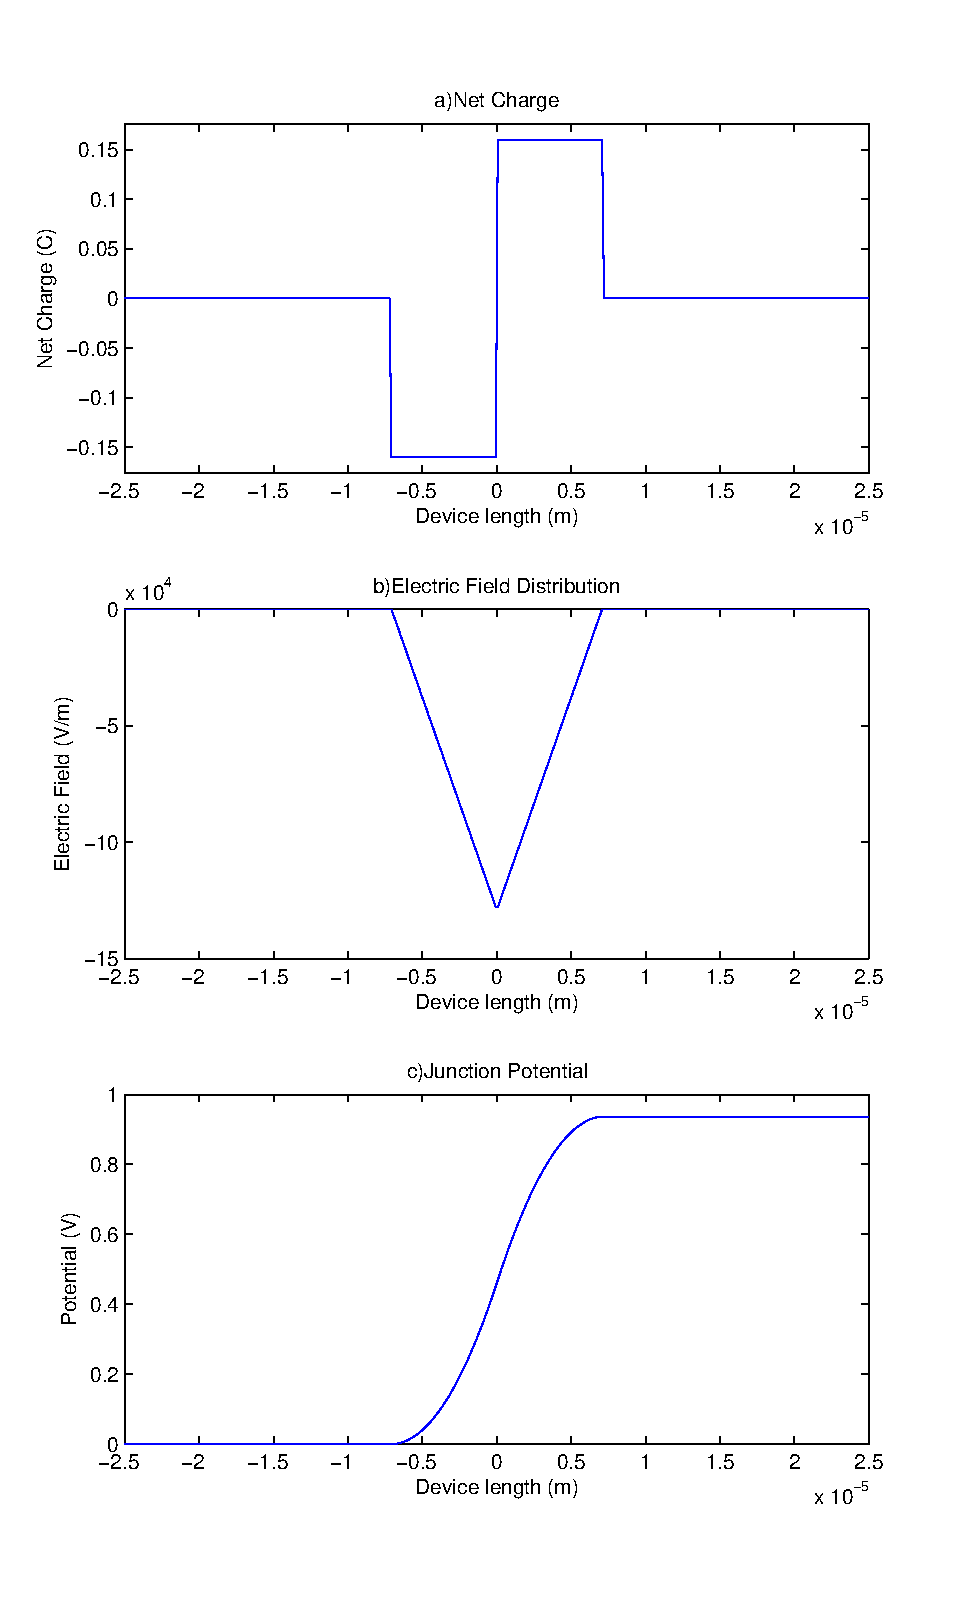
\includegraphics[scale=0.6]{3332}
\caption{Approximate Solution of a PN Junction} 
\label{pnplt}
\end{figure}

\end{doublespace}

